\documentclass[a4paper, 11pt]{article}

\newcommand{\templates}{../../template}
\usepackage[a4paper, margin=2.5cm]{geometry}

\usepackage{enumitem}
\setlist[itemize]{noitemsep}
\setlist[enumerate]{noitemsep}

\let\oldpar\paragraph
\renewcommand{\paragraph}[1]{\oldpar{#1\\}\noindent}

% Avoid dots in the table of contents, it mess with the gulpease calculation
\makeatletter
\renewcommand{\@dotsep}{10000} 
\makeatother
\usepackage{graphicx}
\usepackage{hyperref}
\usepackage{makecell}
\usepackage{fancyhdr}

\newcommand{\settitolo}[1]{\newcommand{\titolo}{#1\\}}
\newcommand{\setprogetto}[1]{\newcommand{\progetto}{#1\\}}
\newcommand{\setcommittenti}[1]{\newcommand{\committenti}{#1\\}}
\newcommand{\setredattori}[1]{\newcommand{\redattori}{#1\\}}
\newcommand{\setrevisori}[1]{\newcommand{\revisori}{#1\\}}
\newcommand{\setresponsabili}[1]{\newcommand{\responsabili}{#1\\}}
\newcommand{\setversione}[1]{
	\ifdefined\versione\renewcommand{\versione}{#1\\}
	\else\newcommand{\versione}{#1\\}\fi
}
\newcommand{\setdestuso}[1]{\newcommand{\uso}{#1\\}}
\newcommand{\setdescrizione}[1]{\newcommand{\descrizione}{#1\\}}

\newcommand{\makefrontpage}{
	\begin{titlepage}
		\begin{center}

		
\includegraphics[width=0.4\textwidth]{\templates/4ourSquared_logo}\\

		{\Large 4OURSQUARED}\\[6pt]
		\href{mailto://4oursquared.unipd@gmail.com}{4oursquared.unipd@gmail.com}\\
		
		\ifdefined\progetto
		\vspace{1cm}
		{\Large\progetto}
		{\large\committenti}
		\else\fi
		
		\vspace{1.5cm}
		{\LARGE\titolo}
		
		\vfill
		
		\begin{tabular}{r | l}
		\multicolumn{2}{c}{\textit{Informazioni}}\\
		\hline
		
		\ifdefined\redattori
			\textit{Redattori} &
			\makecell[l]{\redattori}\\
		\else\fi
		\ifdefined\revisori
			\textit{Revisori} &
			\makecell[l]{\revisori}\\
		\else\fi
		\ifdefined\responsabili
			\textit{Responsabili} &
			\makecell[l]{\responsabili}\\
		\else\fi
		
		\ifdefined\versione
			\textit{Versione} & \versione
		\else\fi
		
		\textit{Uso} & \uso
		
		\end{tabular}
		
		\vspace{2cm}
		
		\ifdefined\descrizione
		Descrizione
		\vspace{6pt}
		\hrule
		\descrizione
		\else\fi
		\end{center}
	\end{titlepage}
}
\usepackage{hyperref}
\usepackage{array}
\usepackage{tabularx}
\usepackage{adjustbox}

\newcounter{verscount}
\setcounter{verscount}{0}
\newcommand{\addversione}[5]{
	\ifdefined\setversione
		\setversione{#1}
	\else\fi
	\stepcounter{verscount}
	\expandafter\newcommand%
		\csname ver\theverscount \endcsname{#1&#2&#3&#4&#5}
}

\newcommand{\listversioni}{
	\ifnum\value{verscount}>1
		\csname ver\theverscount \endcsname
		\addtocounter{verscount}{-1}
		\\\hline
		\listversioni
	\else
		\csname ver\theverscount \endcsname\\\hline
	\fi
}

\newcommand{\makeversioni}{
	\begin{center}
		\begin{tabularx}{\textwidth}{|c|c|c|c|X|}
		\hline
		\textbf{Versione} & \textbf{Data} & \textbf{Redattore} & \textbf{Verificatore} & \textbf{Descrizione} \\
		\hline
		\listversioni
		\end{tabularx}
	\end{center}
	\clearpage
}

\usepackage{graphicx}
\usepackage{float}
\graphicspath{{img/}}

\settitolo{Specifica Tecnica}
\setprogetto{Lumos Minima}
\setcommittenti{Imola Informatica}
\setredattori{Soldà Matteo}
\setdestuso{esterno}
\setdescrizione{
Questo documento descrive la specifica architetturale del progetto, illustrando gli aspetti progettuali che caratterizzino il design del prodotto.
}

\addversione{0.0.0}{05/09/2023}{Soldà Matteo}{Alberti Nicolas}{Prima stesura.}
\addversione{0.0.1}{20/09/2023}{Soldà Matteo}{Alberti Nicolas}{Stesura delle prime sezioni.}
\begin{document}
\makeindexdetails
\makefrontpage \makeversioni
\tableofcontents
\newpage
\listoffigures
\clearpage
\makecontentsdetails{Specifica Tecnica}
\newpage
\section{Introduzione}
\subsection{Scopo del Documento}
Questo documento ha lo scopo di descrivere nel dettaglio, sopratutto tramite diagrammi, le caratteristiche architetturali del prodotto software sviluppato.
\subsection{Riferimenti Normativi}
\begin{itemize}
    \item \href{https://www.math.unipd.it/~tullio/IS-1/2022/Progetto/C2.pdf}{Capitolato C2 - Lumos Minima}
\end{itemize}

\subsection{Riferimenti Informativi}
\begin{itemize}
    \item \href{https://www.math.unipd.it/~rcardin/swea/2022/Software%20Architecture%20Patterns.pdf}{Design Pattern Architetturali}
    \item \href{https://www.math.unipd.it/~rcardin/swea/2022/Design%20Pattern%20Architetturali%20-%20Dependency%20Injection.pdf}{Dependency Injection}
    \item \href{https://www.math.unipd.it/~rcardin/sweb/2022/L02.pdf}{MVC e Derivati}
    \item \href{https://www.math.unipd.it/~rcardin/swea/2022/Design%20Pattern%20Creazionali.pdf}{Pattern Creazionali}
    \item \href{http://www.math.unipd.it/~tullio/IS-1/2006/Approfondimenti/SEI-Software_Architectures.pdf}{Software Architecture}
    \item \href{https://www.math.unipd.it/~rcardin/swea/2022/Design%20Pattern%20Strutturali.pdf}{Pattern Strutturali}
    \item \href{https://www.math.unipd.it/~rcardin/swea/2021/Design%20Pattern%20Comportamentali_4x4.pdf}{Pattern Comportamentali}
    \item \href{https://www.math.unipd.it/~rcardin/swea/2021/SOLID%20Principles%20of%20Object-Oriented%20Design_4x4.pdf}{Programmazione SOLID}
\end{itemize}

\newpage
\section{Tecnologie Utilizzate}
\subsection{Frontend}
Per realizzare il frontend, ossia la parte di applicazione che viene eseguita sul browser dell'utente, sono state utilizzate le seguenti tecnologie:
\begin{itemize}
    \item React: libreria JavaScript per la creazione di interfacce utente;
    \item Typescript: linguaggio di programmazione che estende JavaScript aggiungendo i tipi, permettendo una codifica più robusta e sicura;
    \item Bootstrap: framework CSS per la creazione di interfacce responsive e accattivanti;
\end{itemize}
\subsection{Backend}
Per realizzare il backend, ossia la parte di applicazione che viene eseguita sul server, sono state utilizzate le seguenti tecnologie:
\begin{itemize}
    \item Node.js: runtime JavaScript che permette di eseguire codice JavaScript lato server;
    \item Typescript: linguaggio di programmazione che estende JavaScript aggiungendo i tipi, permettendo una codifica più robusta e sicura;
    \item Express: framework che permette di creare applicazioni web e API più facilmente e con una miglior gestione;
    \item Axios: client HTTP basato su promise per effettuare richieste HTTP basate su Promise;
    \item Mongoose: libreria che permette di gestire in modo più semplice e intuitivo i database MongoDB;
    \item Cors: middleware che permette di configurare in modo semplice e veloce le politiche CORS;
    \item JWT: libreria che permette di gestire in modo semplice e veloce i token JWT;
    \item Cron: libreria che permette di gestire in modo semplice e veloce i cronjob, ossia per la creazione di routine automatiche;
\end{itemize}

\subsection{Database}
Il database utilizzato è di tipo NoSQL, in particolare MongoDB, che permette di gestire documenti in formato BSON (Binary JSON).\\

\subsection{Meccanismo di Comunicazione}
Tutte le comunicazioni, sia esterne (da client a server) che interne (da server a server) sono state gestite tramite API REST.\\

\newpage
\section{Architettura Logica}
\subsection{Frontend}
\begin{figure}[H]
    \centering
    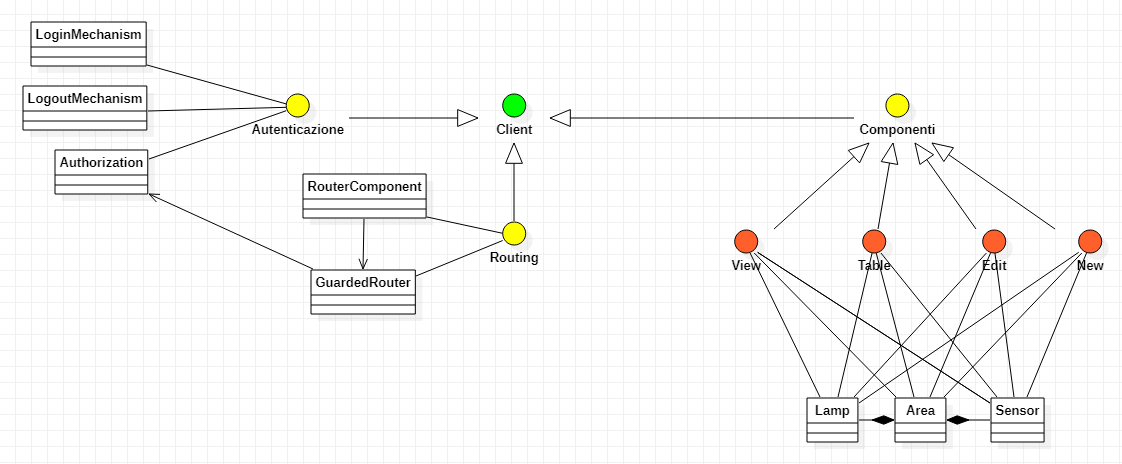
\includegraphics[width=\textwidth]{ArchitetturaClient}
    \caption{Architettura del client.}
\end{figure}
\subsection{Backend}
\begin{figure}[H]
    \centering
    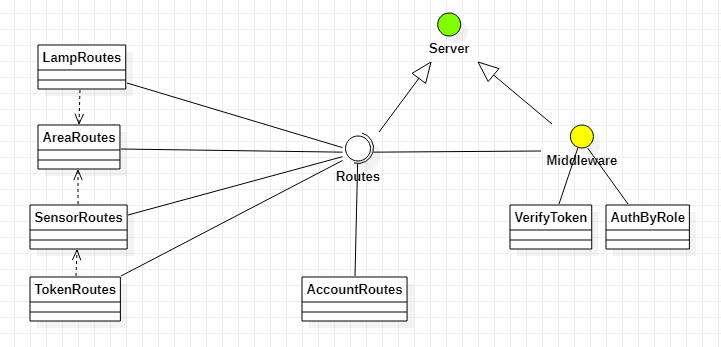
\includegraphics[width=\textwidth]{ArchitetturaServer}
    \caption{Architettura del server.}
\end{figure}

\newpage
\section{Design Pattern}
Lumos Minima è un'applicazione web di tipo SPA (Single-page application) per la gestione di impianti luminosi e di sensori per la rilevazione del movimento associati ai primi, raggruppati in insiemi definiti aree illuminate.\\
L'applicazione si avvale del cosiddetto stack MERN (dove le iniziali stanno rispettivamente per MongoDB, Express.JS, React.JS, Node.JS) e presenta un design architetturale “3-tier” dotata di un comparto client (presentazione), un server (“business logic”), e un database No-SQL per ospitare i dati (persistance). Tuttavia, invece di JavaScript “puro” si è preferito TypeScript, che viene compilato in JavaScript e fornisce un supporto opzionale della tipizzazione stretta. Il diagramma mostra le tecnologie di cui si serve ciascun layer.
\begin{figure}[H]
    \centering
    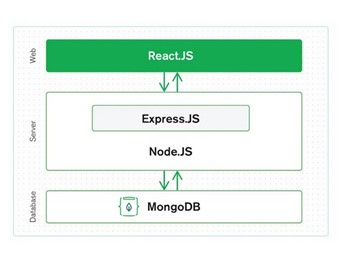
\includegraphics[width=\textwidth]{MERN}
    \caption{Rappresentazione grafica dell'architettura MERN.}
\end{figure}
Questo sistema “a livelli” è stato scelto poiché, oltre a trattarsi di un sistema consolidato (e quindi che si prestasse a uno sviluppo anche gravato da vincoli temporali stringenti), consente in modo agevole il mock del layer sottostante in occasione dei test di unità, vista la necessità di raggiungere la percentuale di code coverage inizialmente indicata nel capitolato.

\newpage
\section{Altri Aspetti Progettuali Rilevanti}
\subsection{Persistenza dei Dati}
Per realizzare lo strato di persistenza dei dati, come precedentemente indicato, è stato utilizzato MongoDB, un database NoSQL che permette di gestire documenti in formato BSON (Binary JSON).\\
\begin{figure}[H]
    \centering
    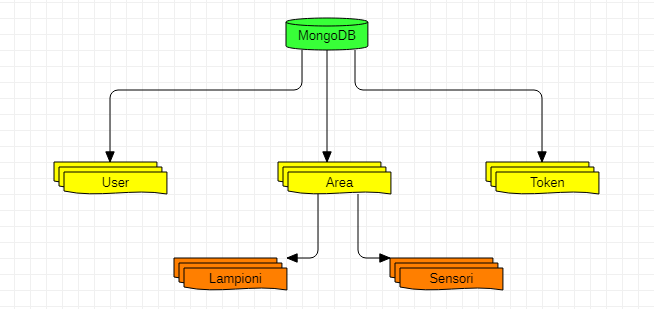
\includegraphics[width=\textwidth]{Persistenza}
    \caption{Struttura del database.}
\end{figure}
A differenza di un database di tipo SQL, in MongoDB, i dati sono raccolti in \textit{collezioni}. Queste \textit{collezioni} contengono uno, nessuno o una moltitudine di \textit{documenti}.\\
Dato che nei database di tipo NoSQL non esiste il concetto di "relazione", ogni documento di tipo area conterrà un array di documenti di tipo sensore e un array di documenti di tipo lampione.\\\\
Per quanto riguarda invece la comunicazione tra il server e il database, per poter comunicare i dati tra una parte e l'altra, sono stati utilizzati gli schemi di \textit{Mongoose} che permettevano di definire la struttura dei dati, i tipi di dati, i vincoli e le validazioni, oltre a fornire una interfaccia che permettesse di comunicare con il giusto tipo di dati.\\
Di seguito la struttura dei documenti (e conseguentemente degli schemi) utilizzati:
\begin{figure}[H]
    \centering
    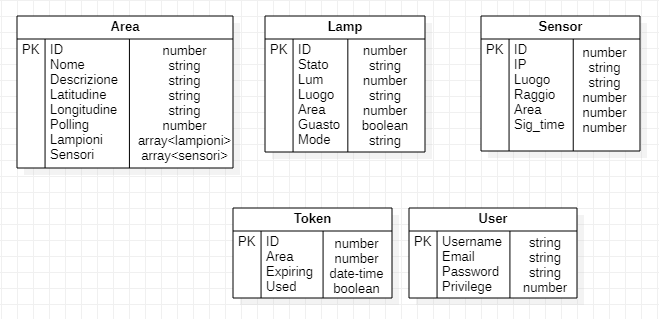
\includegraphics[width=\textwidth]{SchemaDB}
    \caption{Struttura dei dati nel DB.}
\end{figure}

\subsection{Interfacciamento tra Sensori e Lampioni}
Per accedere ai dati riguardanti un determinato lampione e/o sensore, abbiamo utilizzato la lettura di parametri dalla URL.\\ Ovviamente gli endpoint relativi ai sensori e ai lampioni sono distinti, infatti:
\begin{itemize}
    \item Endpoint sensori: \textit{/api/aree/$<$IdArea$>$/sensori/$<$IdSensore$>$};
    \item Endpoint lampioni: \textit{/api/aree/$<$IdArea$>$/lampioni/$<$IdLampione$>$};
\end{itemize}
\subsection{Comunicazione Automatica}
Per quanto riguarda il meccanismo che permette di aumentare e diminuire automaticamente la luminosità dei lampioni che si trovano dentro una determinata area illuminata, il soggetto principale sono i sensori: essi, qualora rilevassero il movimento di una persona, di un veicolo o di un animale, dovrebbero inviare una richiesta di tipo HTTP all'endpoint prestabilito. Alla ricezione della richiesta, il server si occuperà della gestione della stessa come descritto nel diagramma sottostante.
\begin{figure}[H]
    \centering
    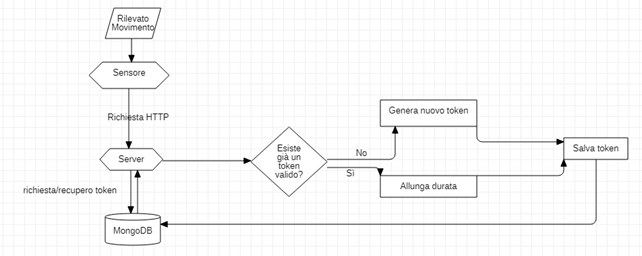
\includegraphics[width=\textwidth]{sensori}
    \caption{Diagramma di flusso del segnale relativo al movimento rilevato dai sensori.}
\end{figure}
Il token trova un utilizzo concreto solo per i lampioni dell'area che sono configurati in modalità PULL (manuale).\\ 
Per questo motivo, di seguito c'è una piccola spiegazione di come viene gestito il rilevamento di movimento da entrambi i tipi di lampione:
\begin{itemize}
    \item PUSH: i lampioni si illuminano quando il sensore segnala un movimento, senza necessità di utilizzare il token
    \item PULL: la parte di server vhe gestisce l'area illuminata, con cadenza regolare e definita dall'atributo \textit{polling time}, controlla nel database se c'è un token valido per l'area di riferimento:
    \begin{itemize}
        \item Se il token è valido e inutilizzato: illumina tutti i lampioni impostati in modalità PULL;
        \item Se il token non è valido ma è stato utilizzato: riduce la luminosità di tutti i lampioni a quella iniziale;
        \item Negli altri casi, verrà restituito un codice stato consono, ma senza effettuare nessun'altra azione.
    \end{itemize}
\end{itemize}

\subsection{Autenticazione e Autorizzazione tramite JWT}
Dopo aver inserito le proprie credenziali nella login mask, se la password (criptata con hashing SHA512) coincide con quella dell'utente viene restituito un token JWT firmato dal server, una stringa che contiene informazioni sul ruolo dell'utente. L'autorizzazione (necessaria per l'accesso alle pagine dal lato “client”, e per utilizzare le API del server) sfrutta questo meccanismo:
\begin{figure}[H]
    \centering
    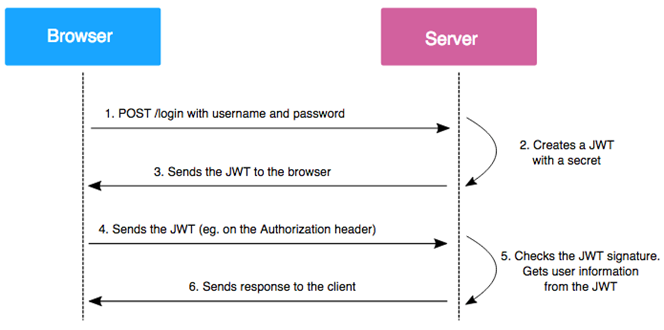
\includegraphics[width=\textwidth]{auth}
    \caption{Diagramma di flusso del meccanismo di autorizzazione tramite JWT.}
\end{figure}

Tuttavia, il JWT è memorizzato (e inviato al server) all'interno di un cookie HTTP-Only: questo impedisce che il contenuto del cookie possa essere letto da codice JavaScript malevolo, vanificando così attacchi alla confidenzialità di tipo XSS (Cross-Site Scripting).\\\\
Le API sono protette da due livelli di middleware che prendono in carico la richiesta HTTP.
\begin{figure}[H]
    \centering
    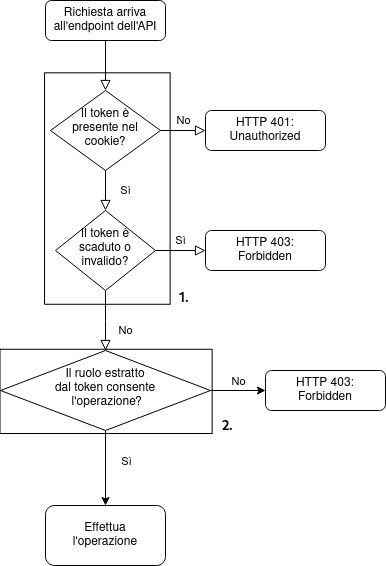
\includegraphics[width=\textwidth]{middleware}
    \caption{Diagramma di flusso del meccanismo di autorizzazione tramite middleware.}
\end{figure}

\end{document}